\documentclass[11pt, letterpaper, oneside]{book}
\usepackage[left=1.5in, right=1.5in, bottom=1in, top=1.6in]{geometry}
\usepackage{amsfonts}  %fonts like \mathbb{}
\usepackage{amssymb,amsmath}
\usepackage{graphicx}
\usepackage{mathrsfs} %for \mathscr
%\usepackage[colorlinks=true,urlcolor=blue,linkcolor=blue]{hyperref} % navega por el doc
\usepackage{hyperref} %hyperref of equations

\title{Lectures on General Relativity}
\author{Juan Guarin, Antonio Calixto}
\date{August, 2023}

\def\Re{\mathbb{R}}

\begin{document}
%\maketitle
\begin{center}
	\huge \textbf{Lectures on General Relativity}
	
	\vspace{5mm}
	By: Juan Andrés Guarín-Rojas,\\
	Antonio Calixto Gutiérrez-Piñeres
	
	\vspace{5mm}
	August 30th, 2023
\end{center}
\vfill
\begin{figure}[hb]
	\centering
	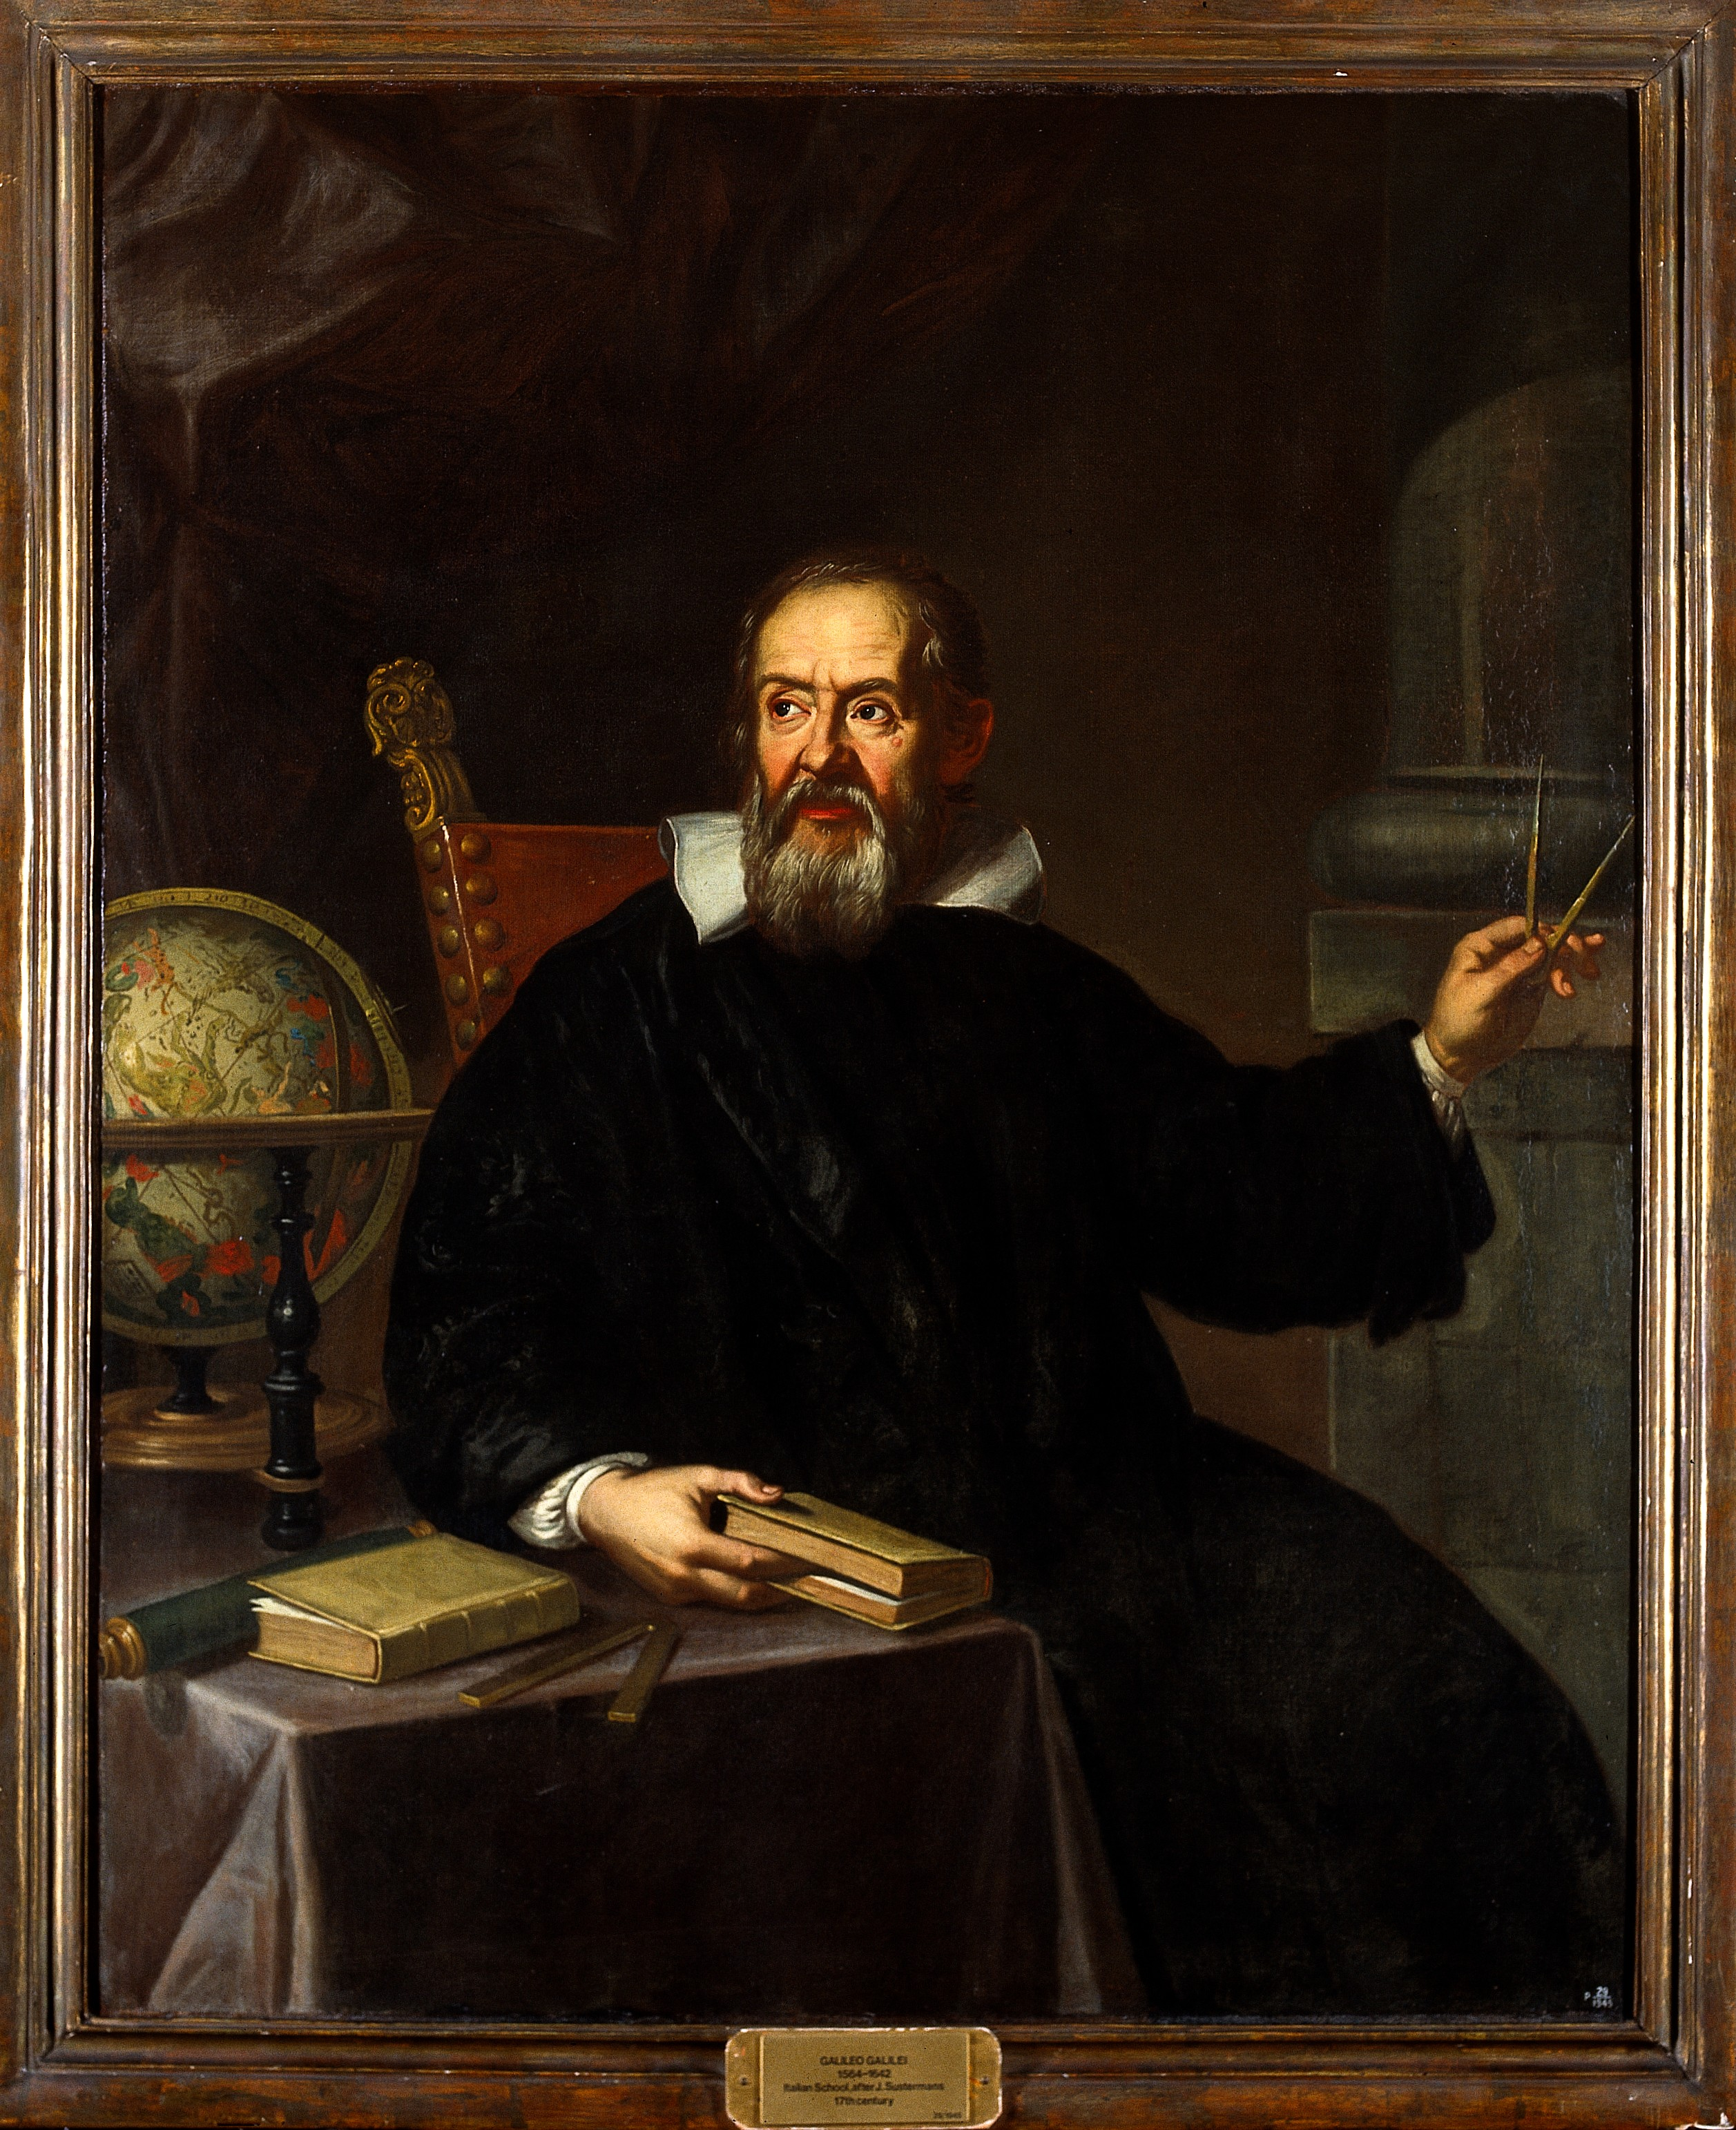
\includegraphics[width=0.8\linewidth]{images/Galileo-Galilei.jpg}
\end{figure}
\vfill

\newpage

\textit{Was du ererbt von deinen Vätern hast, Erwirb es, um es zu besitzen}

\rule{\linewidth}{0.4pt}
\begin{flushright}
\textsc{goethe}
\end{flushright}
%\noindent
\begin{figure}[ht]
	\centering
	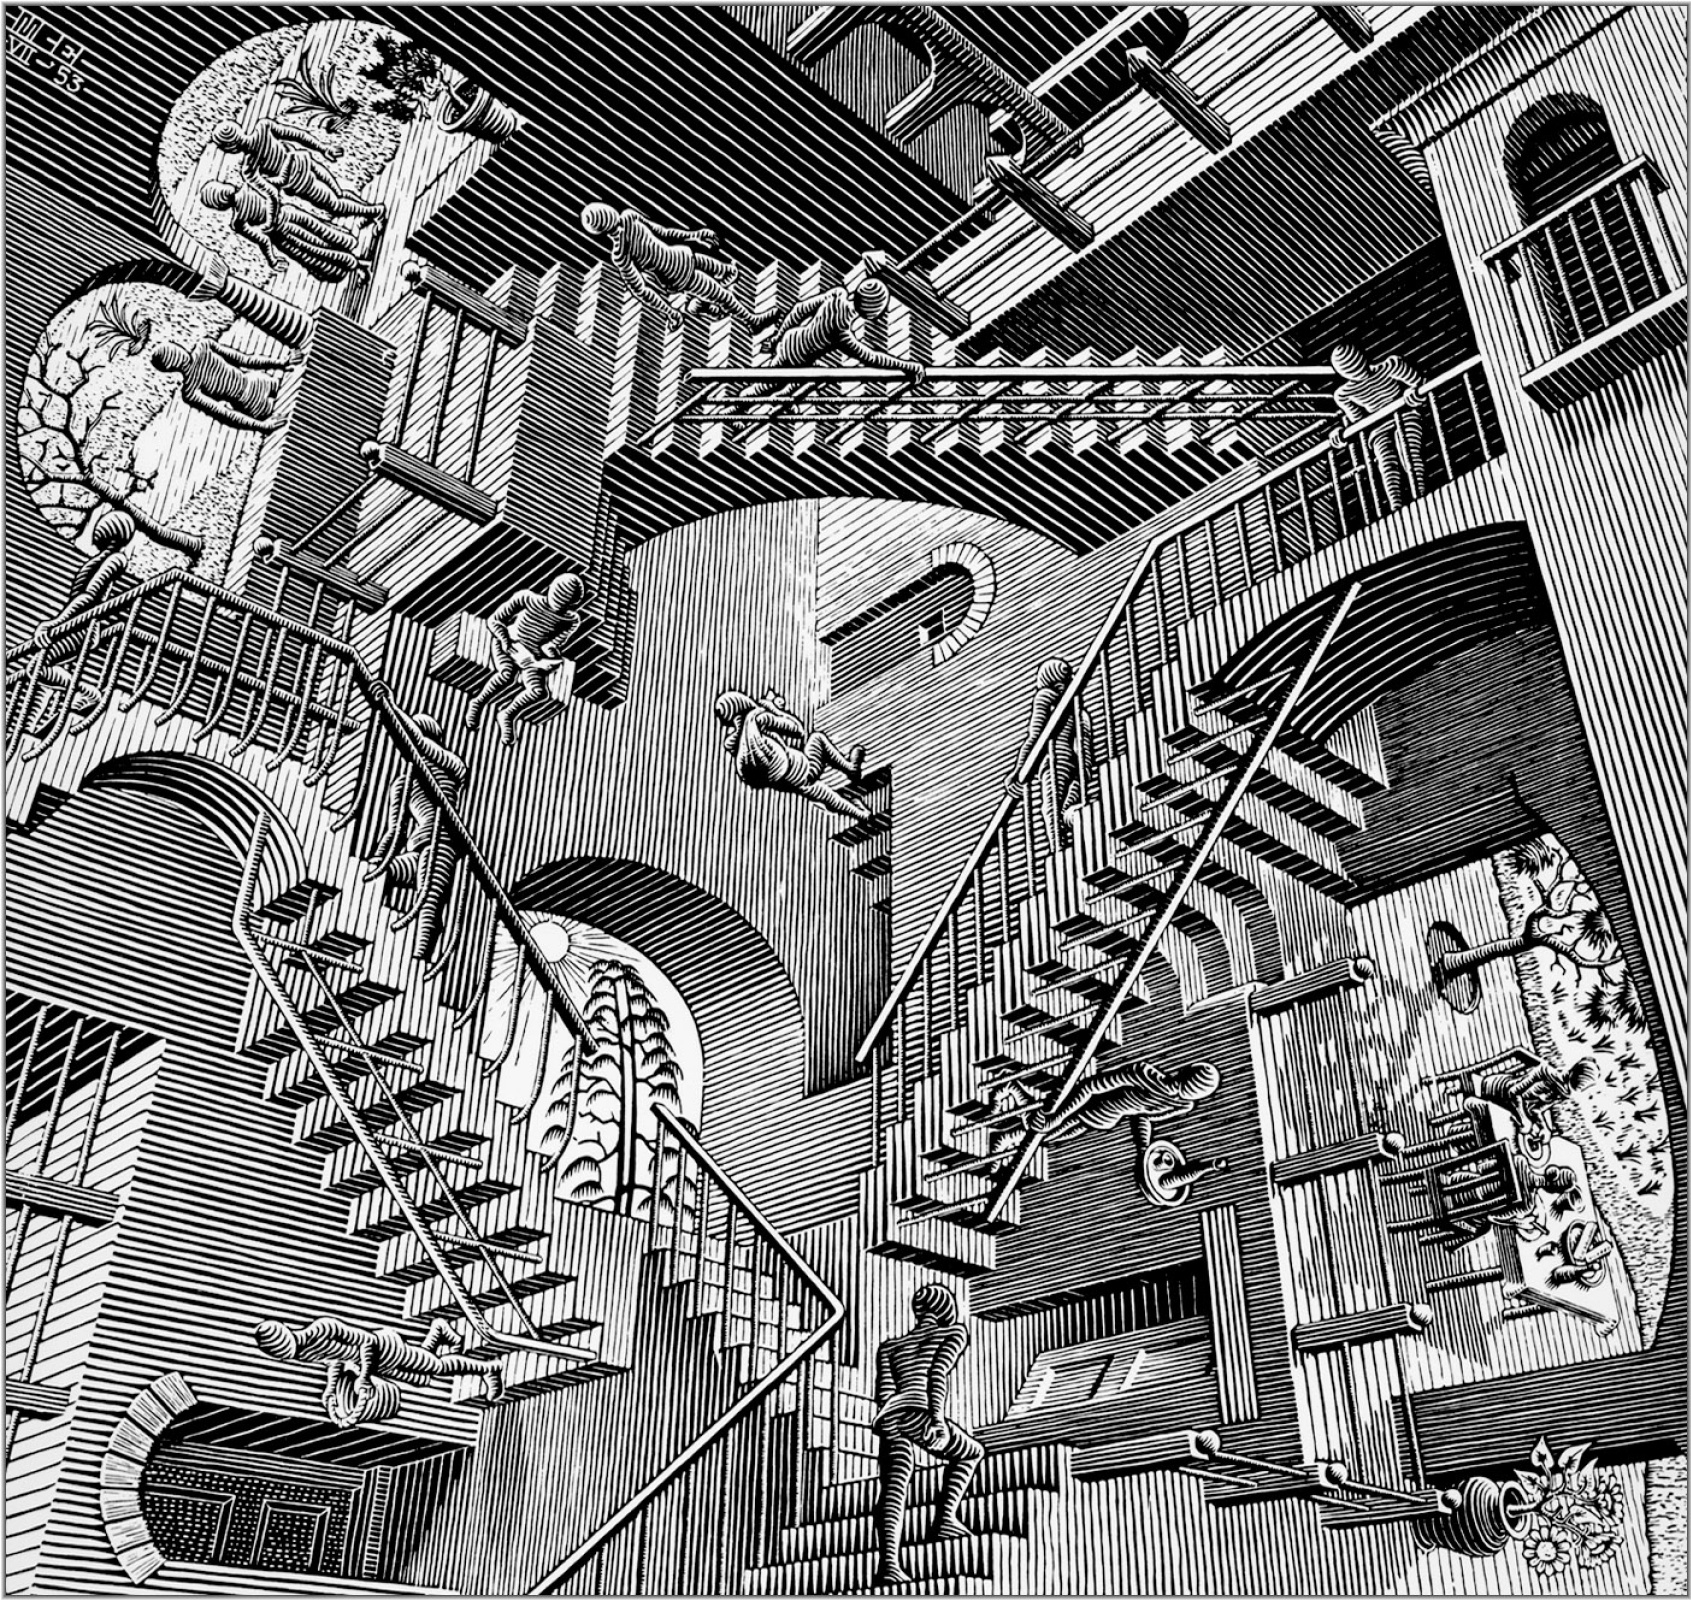
\includegraphics[width = 0.8\linewidth]{images/relatividad_escher.jpg}
	\caption{\textit{Relatividad} por M.C. Escher (1953).}
\end{figure}

\tableofcontents

\chapter{Invariance vs covariance}
We would discuss how the concepts of \textit{invariance} and \textit{covariance} are present in Classical mechanics, Special Relativity and General Relativity. We would figure it out the intrinsic relation between invariance and covariance, and how they are used in physics theories mentioned above.

\section{Fundamental concepts}
\subsection{Mathematical notion of invariance}
We defyne the mathematical notion of invariance as
\begin{itemize}
	\item[] \textsc{invariance of an object}\\
	\textit{A mathematical object or property of an object is said to be invariant if it do not change under some kind of transformations.}
	
\end{itemize}

In particular, we can say that an object is invariant respecting to a specific transformation, e.g. the invariance of a lattice of points under a translation or rotation of space must be called: translation invariance or rotation invariance respectively. The transformations also can be part of a group of transformations, in which case we can say that the mathematical object is invariant under the group of transformations.

It is also important to say that for transformation we means just some function $T$ that takes any objec (or part of an object or a basis structure where the object is defined) that belongs to a set $O$ and carry it to the same or any other set $O^*$. And, for \textit{kind of transformations} we mean that there exits an equivalence class that join together the transformations in one set, such that the object is invariant under the elements of that set of transformations.

\subsection{Physicall notion of covariance}
In math the notion of covariance is related to how an object such as the components of a covector change under some transformation such as change of basis. But in physics this term is usually use for a specific kind of invariance, that is that the structure of an equation remains the same after some coordinate transformation. As for example, an equation like $\vec{F}=m\vec{a}$ will be invariance if, after make a transformation of coordinates to another frame, it has de form $\vec{F}\,'=m\vec{a}\,'$, where $\vec{F}\,'$ and $\vec{a}\,'$ are objects defined the same as $\vec{F}$ and $\vec{a}$ but for the primed reference frame.

So, we define covariance as
\begin{itemize}
	\item[] \textsc{Covariance of a law of physics under a set of transformations $\mathcal{T}$}\\
	\textit{Any equation of a law of physics is said to be covariant if its structure remain the same after making a transformation of $\mathcal{T}$}	
\end{itemize}

The set of transformations can form a group, for example with composition operation, and also can be a set of coordinate transformations. For transformation we mean the same as the previous section.

The covariance is present in theories of physics as in the Galilean Invariance, the Lorentz Invariance and the General Covariance of the laws of General Relativity.

\section{The idea behind Equivalence Principle}
Gauss assumes that in every point of a surface is always possible to choose a cartesian system of coordinates wich satisfies euclidian geometry locally, for a small neighbourhood of the point. This idea extends to any hypersurface in the Riemmannian geometry. The initial assumption of Gauss implies that is possible to entirely know the curvature of a surface with the function of transformation of the cartesian coordinates $\xi$ to the surface coordinates $x$. This is analog to the Equivalence Principle in which is possible to determine all the effects of gravitational field in terms of the field equation of an inertial coordinate system $\xi$ extendended to a general system of coordinates $x$, by using the metric  $g_{\mu,\nu}$ and the connection $\Gamma^{\gamma}\,_{\mu \nu}$ that depends on the metric and the connection for the inertial system through the transformation rule of coordinates $\xi^\alpha(x^\mu)$.

$$\Gamma^\lambda\,_{\mu\nu} = \frac{\partial x^\lambda}{\partial \xi^\alpha}\frac{\partial^2\xi^\alpha}{\partial x^\mu \partial x^\nu}$$

$$g_{\mu\nu}=\frac{\partial \xi^\alpha}{\partial x^\mu} \frac{\partial \xi^\beta}{\partial x^\nu} \eta_{\alpha\beta}$$

We note from this the essence of the kind of invariance that is present in General Relativity, that is that when we pass to an equation valid for a local inertial system (of Special Relativity) to its form for a general system then the metric and the affine connection come up, in such a way, the new equation is a tensorial equation that preservs its structure or form under general coordinate transformations $x^\mu \to x'^\mu$.

As an example, following \cite{weinberg}, for a weak static field generated by nonrelativistic matter in a inertial system we have
\begin{equation}
	\nabla^2g_{00}=-8\pi GT_{00} \label{eq:field-intertial-system}
\end{equation}
that is obtained based on the Newtonian potential $\phi$ determined by Poisson's equation ${\nabla^2 \phi = 4\pi G \rho}$, where $\rho$ is the mass density. Equation \ref{eq:field-intertial-system} allows to guess that the field equation for the inertial system is of the form
\begin{equation}
	G_{\alpha\beta} = -8\pi GT_{\alpha\beta}
\end{equation}
where $G_{\alpha\beta}$ is a linear combination of the metric and its first and second derivates. So, from the Principle of Equivalence the equation that govern gravitational fields of arbitrary strength and in a general frame must take the form
\begin{equation}
	G_{\mu\nu} = -8\pi GT_{\mu\nu}
\end{equation}
where $G_{\mu\nu}$ is a tensor that reduces to $G_{\alpha\beta}$ for weak fields. After certain derivations that do not concern here\footnote{For a complete description see \cite{weinberg}} we get
\begin{equation}
	G_{\mu\nu} = R_{\mu\nu}-\frac{1}{2}g_{\mu\nu}R \label{eq:Guv}
\end{equation}
where $R_{\mu\nu}=R^\lambda\,_{\mu\lambda\nu}$ is the Ricci tensor and $R=R^\mu\,_\mu$ is the curvature scalar. Finally, in equation \ref{eq:Guv} we can expect to have terms related to the metric $g_{\mu\nu}$ and the affine connection $\Gamma^\lambda_{\mu\nu}$ that are not present in $G_{\alpha\beta}$ for the local inertial system. Thus, the field equation of gravity differs for a local inertial system (locally Minkowski) related to a general system by the coming up of the metric and the affine connection. On the next section we will see that the Principle of Special Relativity and the Galileo's Principle Relativity of the invariance of the law of physics are preciesly characterized by the fact that nothing comes up or disappear while changing from one inertial system to another. In the present case, equation \ref{eq:field-intertial-system} shows that at least there is one coordinate system in wich the metric becomes $\eta_{\alpha\beta}$ and the affine connection becames zero $\Gamma^\lambda\,_{\alpha\beta}=0$. We will come back to analyze this fact when we will talk about the Principle of General Covariance.

\section{Galileo's Principle of Relativity}
Galileo's Principle of Relativity can be statement in the form\footnote{See for example \cite{arnold}}

\textit{There exist coordinate systems, called intertial, possesing the following properties:}
\begin{itemize}
	\item[\textit{1}] \textit{All the laws of the nature at all moments of time are the same in all inertial coordinate systems.}
	\item[\textit{2}] \textit{All coordinate systems in uniform rectilinear motion with respect to an inertial one are themselves inertial.}
\end{itemize}

Here we want to point out what it means for the laws of physics that they \textit{are the same} in all inertial coordinate systems. For this we means that the law of physics is invariant under the action of the Galileo's group, which is that the law equations keep its form under a Galilean transformation $T$ that belongs to the Galilean group $\mathscr{G}$.

The Galilean group $\mathscr{G}$ is defined as the set of invertible affine transformations of the four-dimensional affine space $A^4$ that represents the Newtonian spacetime. The group operation is composition of transformations. To belong to the Galilean group, a transformation ${T:A^4\to A^4}$ must preserve the time interval of any pair of events and preserve the distance between two simoultaneous events, that is
\begin{itemize}
	\item[1.] $\Delta  t_{pq} = \Delta t_{T(p)T(q)}
$ for any $p$ and $q$ in $A^4$.
	\item[2.] If $p$ and $q$ are in $A^4$, and $\Delta t_{pq}=0$ then $||\overrightarrow{pq}||=|| \overrightarrow{T(p)T(q)}||$
\end{itemize}

where $\Delta t_{pq}$ depends on a non-zero linear form $\tau:\Re^4\to\Re$ such that $\Delta t_{pq}:=\tau(\overrightarrow{pq})$, and $||.||$ is a norm that depends on an inner product $\left<.,.\right>$ defined on the kernel subspace of $\tau$.

There exists 10 independently transformations of this kind that are basis for the Galilean group, we clasify them in three classes
\begin{enumerate}
	\item \textsc{uniform motion with velocity} $\vec{v}$
	$$g_1((t,\vec{x}))=(t,\vec{x}+\vec{v}t)\, , \, \vec{v}\in\Re^3$$
	\item \textsc{translation of the origin $(0,0)$ to $(s,\vec{w})$}
	$$g_2((t,\vec{x}))=(t+s,\vec{x}+\vec{w})\, , \, (s,\vec{w})\in\Re\times\Re^3 $$
	\item \textsc{Rotation $R$ of the coordinate axis}
	$$g_3((t,\vec{x}))=(t,R\vec{x})\, , \, R\in SO(3,\Re)$$
\end{enumerate}

where here $(t,\vec{x})\in \Re\times\Re^3$, and $SO(n,\Re)$ holds for the special orthogonal group of $n\times n$ orthogonal matrices with determinant equals to 1 and with reals entries. The $SO(n,\Re)$ group has dimension of $n(n-1)/2$. Is left as an excersice to the read prove that this transformations belongs to the Galilean group. 

We note that a general Galilean transformation is of the form
\begin{equation}
	T(t,\vec{x})=(t+s,R\vec{x}+\vec{u}t+\vec{w})\,,\, s\in\Re\,,\,\vec{u},\vec{w}\in\Re^3\,,\,R\in SO(3,\Re) \label{eq:generalT}
\end{equation}
so acording to the Galileo's Principle of Relativity the laws of physics must remain the same under coordinate transformations $(t,\vec{x})\mapsto (t',\vec{x}')$ that in case of Newtonian physics are the Galilean transformations. This kind of invariance is that we call covariance, wich express specificly that the structure\footnote{This idea of covariance is present in all classical physics. In GR exists the Principle of General Covariance that uses this idea as is discussed in \cite{weinberg}} of the equation remains the same. We define then
\begin{itemize}
	\item[] \textsc{galilean invariance of a law of physics}\\
	\textit{Any equation of a law of physics that preserve its form under Galilean transformations, and that the transformed equation in its reduced form do not involves quantities related to the original frame is called Galilean invariant}.

The term \textit{reduced form} means that the equation has been manipulated algebraiclly in order to simplify, reduce and elimante terms, such as quantities present in the transformation itself.

\end{itemize}

\subsection{Example 1. Newton's second law for a single particle in a scalar potential}

For clarify this ideas we will do an example. Let us take the Newton's second law for a system of a single particle
\begin{equation}
	\vec{F}=\dot{\vec{p}} \label{eq:F = dot p}
\end{equation}

Let us assume that the particle is inmersed in a scalar potential field $U(||\vec{r}-\vec{r}_0||)$ that depends only in the distance relative to some point $\vec{r}_0$. So that, the Newton's second law of motion converts in
\begin{equation}
	\vec{\nabla}U(||\vec{r}-\vec{r}_0||) = \dot{\vec{p}} \label{eq:2nd Law}
\end{equation}
Now we make a coordinate transformation $\vec{r}\to\vec{r}\,'$ of the form of \ref{eq:generalT} but changing $R\to A$ for have a convenient notation. Firstly, we note that the distance ${R:=||\vec{r}-\vec{r}_0||=||\vec{r}\,'-\vec{r}\,'_0||:=R'}$ remain invariant by definition of Galilean transformation. This implies that the scalar potential remain the same ${U(R)=U(R')}$. Secondlly, for the momentum we get
\begin{equation}
	\frac{d\vec{p}}{dt} = \frac{dm}{dt}\vec{v}+ m\frac{d\vec{v}}{dt} \label{eq:dpdt}
\end{equation}
Then, using the assumption that $m=m'$, by experimental facts for non-relativistic physics, and as $t'=t+s$ with $s$ a constant we have
\begin{equation}
\frac{dm}{dt}=\frac{dm'}{dt'} \underbrace{\frac{dt'}{dt}}_{=1}=\frac{dm'}{dt'} \label{eq:dmdt}
\end{equation}
As $dt=dt'$ we will use the notation $\dot{\vec{a}}$ for the time derivate of a vector field $\vec{a}$ indistinguishably for $t$ and $t'$. For the position vector we have
\begin{equation}
	 \vec{r}\,' = A\vec{r} + \vec{u}t+\vec{w} \label{eq:r}
\end{equation}
\begin{equation}
	\dot{\vec{r}}\,' = A\dot{\vec{r}} + \vec{u} \label{eq:dotr}
\end{equation}
\begin{equation}
	\ddot{\vec{r}}\,' = A\ddot{\vec{r}} \label{eq:ddotr}
\end{equation}
Therefore replacing \ref{eq:dmdt}, \ref{eq:dotr}, and \ref{eq:ddotr} in \ref{eq:dpdt} we obtain
$$	\frac{d\vec{p}}{dt} = \frac{dm'}{dt'}A^{-1}(\vec{v}\,'-\vec{u}) + m'A^{-1} \frac{d\vec{v}\,'}{dt'} $$ 
\begin{equation}
	\frac{d\vec{p}}{dt} = A^{-1}\left( \frac{d\vec{p}\,'}{dt'}-\frac{dm'}{dt'}\vec{u}\right) \label{eq: t dpdt}
\end{equation}
We recall that $A^{-1}$ always exists as each orthogonal matrix has determinant distinct to zero. Thirdly, we focus on the gradient operator $\vec{\nabla}$ acting on $U$. Let us recall that $U$ depends only on the distance $||\vec{r}-\vec{r}_0||=R$, then from vector calculus we know
\begin{equation}
	\vec{\nabla}U(R)=\frac{\partial U}{\partial R}\hat{R}=\frac{\partial U}{\partial R'}\underbrace{\frac{\partial R'}{\partial R}}_{=1} \hat{R}
\end{equation}
\begin{equation}
	\vec{\nabla}U(R) = \frac{\partial U}{\partial R'} \frac{\vec{r}-\vec{r}_0}{|| \vec{r}-\vec{r}_0 ||} \label{eq:grad U}
\end{equation}
Equation \ref{eq:r} holds for every position vector $\vec{r}$ in $\Re^3$, in particular it holds for $\vec{r}_0$
\begin{equation}
	\vec{r}\,'_0 = A \vec{r}_0+\vec{u}t+\vec{w}
\end{equation}
And so, using \ref{eq:r}
\begin{equation}
	\vec{r}\,'-\vec{r}\,'_0 = A(\vec{r}-\vec{r'}) \label{eq:difference r}
\end{equation}
Then, equation \ref{eq:grad U} can be written as
\begin{equation}
	\vec{\nabla} U(R)  = \frac{\partial  U}{\partial R'} A^{-1} \frac{\vec{r}\,'-\vec{r}\,'_0}{|| \vec{r}\,'-\vec{r}\,'_0 ||} = A^{-1} \frac{\partial U(R')}{\partial R'} \hat{R}'=A^{-1}\vec{\nabla}\,'U(R') \label{eq:t nabla U}
\end{equation}
Finally, by equations \ref{eq:t nabla U} and \ref{eq: t dpdt} the Newton's second law of equation \ref{eq:2nd Law} transform as
\begin{equation}
	A^{-1}\vec{\nabla}\,'U(R') = A^{-1}\left( \frac{d\vec{p}\,'}{dt'}-\frac{dm'}{dt'}\vec{u}\right)
\end{equation}
Multiplying the matrix $A$ by left in both sides of equations we have
\begin{equation}
	\vec{\nabla}\,'U(R') = \left( \frac{d\vec{p}\,'}{dt'}-\frac{dm'}{dt'}\vec{u}\right)
\end{equation}

By assuming that the particle do not change its mass $dm' / dt'=0$ and by noting that $\vec{\nabla}\,'U(R')$ is the force in the transformated frame we obtain
\begin{equation}
	\vec{F}\,' = \dot{\vec{p}}\,' \label{eq: F' = dot p'}
\end{equation}

We can see that the equation \ref{eq:F = dot p} keep his form under Galilean transformations (the equation is Galilean invariant), and equally important, it is completely determined by quantities of its own reference frame. It do not involves variables related to another inertial frame, as for example its relative velocity  or relative orientation of axes. In fact, when we develope a Galilean transformation of coordinates as equation \ref{eq:generalT} we expected that the new equation do not depend on the relative velocity to the previous coordinate system, and this is because we want that there woud not exits privileged reference frames for the physics of a phenomenon.

\subsection{Example 2. An equation that is not Galilean invariant}
\label{sec:Example2}
Let us take a charged particle inmerse in a homogeneus and constant magnetic field (see Fig. \ref{fig:cparticle}). The equation of motion of the particle is of the form
\begin{equation}
	\dot{\vec{p}} = q\vec{v}\times \vec{B} \label{eq:motion1}
\end{equation}

We employ a galilean transformation like the equation \ref{eq:generalT}, so we can use equations \ref{eq: t dpdt} and \ref{eq:dotr}
\begin{equation}
	A^{-1} \left( \frac{d\vec{p}\,'}{dt'}-\frac{dm'}{dt'}\vec{u} \right) = q A^{-1}(\vec{v}\,'-\vec{u})\times \vec{B}
\end{equation}

Multiplying both side with A to the left, taking a constant mass, and assuming that the magnetic field change a little $\vec{B} \cong \vec{B}\,'$ we get
\begin{equation}
	\dot{\vec{p}}\,' = q (\vec{v}\,'-\vec{u})\times \vec{B}\,' \label{eq:motion2}
\end{equation}

Obviously, this last equation is not the equation of motion of the charged particle in the new system of reference because we need to consider the electric force, that appears because of the transformation of electromagnetic fields. This derivation is only pedagogical to show one idea. As we can see equations \ref{eq:motion1} and \ref{eq:motion2} differs from the existence of relative velocity vector $\vec{u}$. So, equation \ref{eq:motion1} is not truly Galilean invariant because of this $\vec{u}$ vector. Let see what happen when we apply a second Galilean transformation $T_2$
\begin{equation}
	T_2((t',\vec{r}\,')) =\left(t'+a, D \vec{r}\,'+\vec{\vartheta}t + \vec{b}\right),\, D\in SO(3,\Re)\,,\, \vec{\vartheta},\vec{b}\in\Re^3\,,\,a\in\Re
\end{equation}
If we replace $\vec{r}\,'$ from equation \ref{eq:r}, and $t'=t+s$ we obtain the transformation $T_3$
\begin{equation}
	T_3((t,\vec{r}))= \left(t+\underbrace{(s+a)}_{s^*},\underbrace{DA}_{A^*}\vec{r}+\underbrace{(D\vec{u}+\vec{\vartheta})}_{\vec{u}\,^*}t+\underbrace{(D\vec{w}+\vec{b})}_{\vec{b}\,^*}\right)
\end{equation}
\begin{equation}
	T_3((t,\vec{r})) = \left(t+s^*, A^*\vec{r}+\vec{u}\,^*t+\vec{b}\,^* \right)
\end{equation}
Then, if we transform equation \ref{eq:motion2} in frame $S'$ with $T_2$  it will be like transform equation \ref{eq:motion1} in frame $S$ with $T_3$. This implies that the transformated equation of \ref{eq:motion2} using $T_2$ is
\begin{figure}[ht]
	\centering
	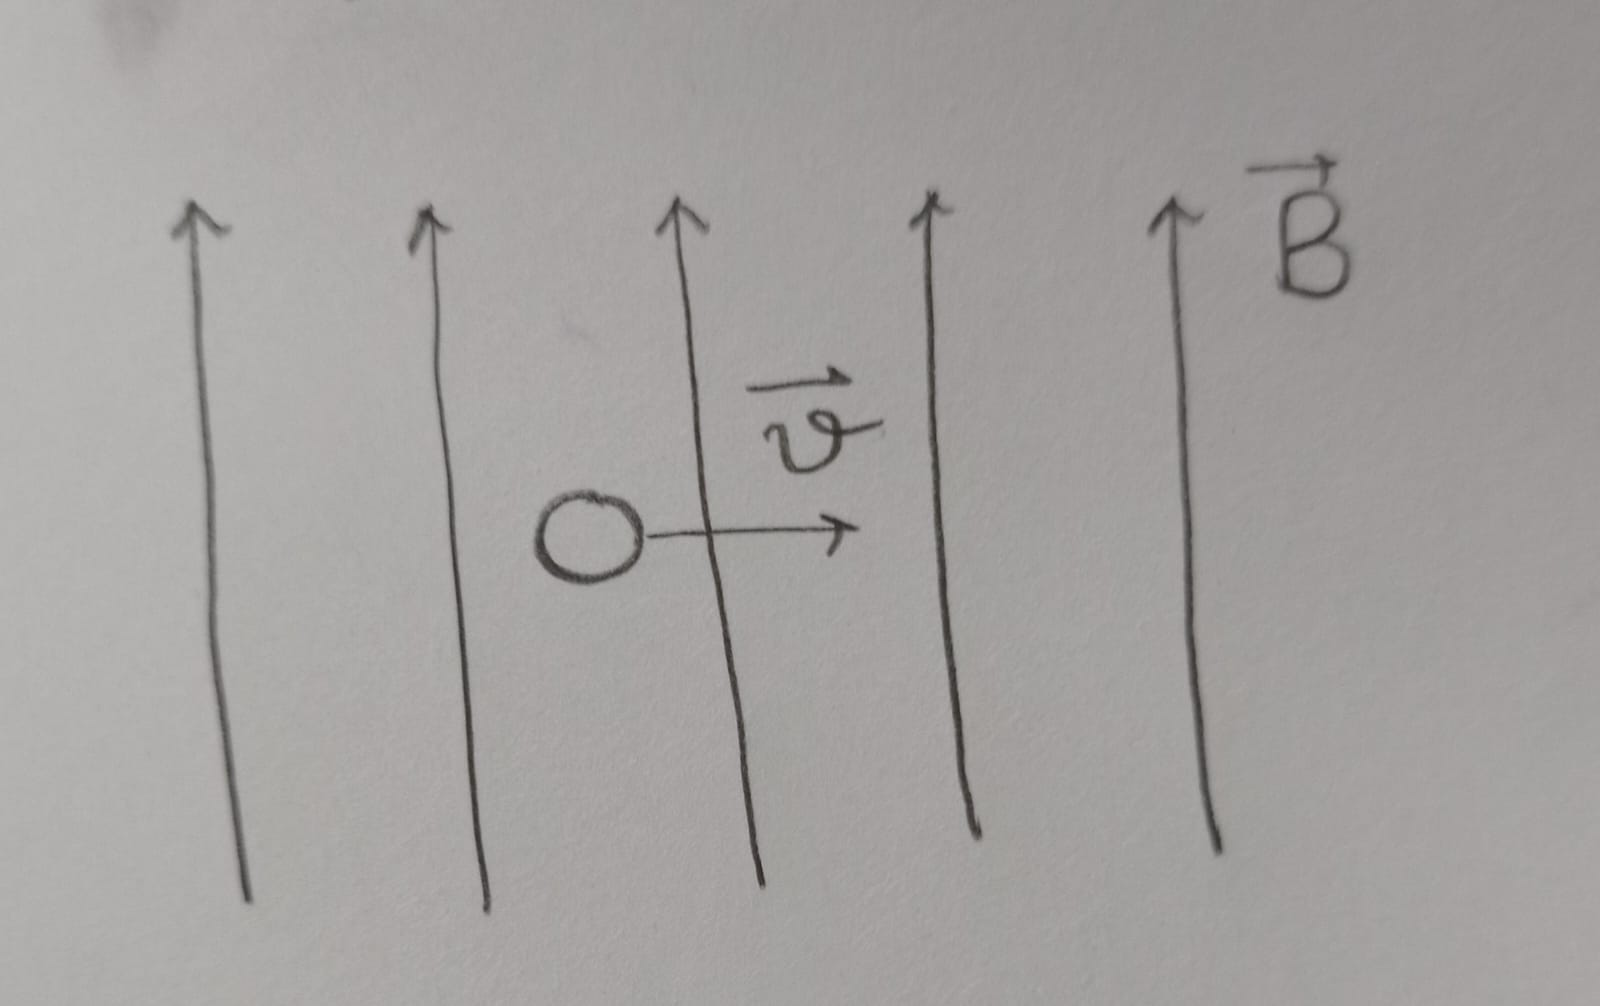
\includegraphics[width = 0.5 \linewidth]{images/charged_particle_homogeneus_B.jpeg}
	\caption{Charged particle in a homogeneous magnetic field $\vec{B}$}
	\label{fig:cparticle}
\end{figure}

\begin{equation}
	\dot{\vec{p}}\,''=(\vec{v}\,''-\vec{u}\,^*)\times \vec{B}\,'' \label{eq:motion3}
\end{equation}
where we also use that $\vec{B}\,''\cong \vec{B}\,'$. Therefore, we see that equation \ref{eq:motion2} is equal to equation \ref{eq:motion3} in structure, being $\vec{u}$ and $\vec{u}\,^*$ the relative velocities of the frames $S'$ and $S''$ to the original one $S$,respectively. By expressing a non Galilean invariant equation as \ref{eq:motion1} in another frame we got a Galilean invariant equation\footnote{This idea of take any equation and see how it looks in other frame, in order to obtain a covariant equation, is presented in chapter 4 of \textit{Weinberg. Gravitation and Cosmology}\cite{weinberg}}. This lead us to think that invariance under Galilean transformation is not the essential part of the Galileo's Principle of Relativity. Actuallt, the key point is that the equation do not concern to relative quantities to other inertial systems besides its covariant itself. General covariance itself is absent of physical content, as any equation can be made generally covariant.

We also note that when $\vec{u}=0$ in \ref{eq:motion1} we recover the original form of the equation in frame $S$. We can say that this equation in fact it is covariant but under the structure of equation \ref{eq:motion1}. This means that if we write \ref{eq:motion1} as 
$$\dot{\vec{p}}=q(\vec{v}-\vec{0})\times \vec{B}$$
then it will be keep this structure under Galilean transformations. This is a covariance in other sense that in the Galileo's Principle of Relativity as we point it out before. This is more likely that a generalized covariance, in the sense that \ref{eq:motion1} is covariant under Galilean transformations althought a velocity vector $\vec{u}$ comes out after the transformation; and that covariance is because we can say that the originally equation \ref{eq:motion1} already have this vector $\vec{u}$ as $\vec{0}$.

\section{Specital Relativity Principle}
The basic postulates of the Special Relativity can be written as\footnote{see \cite{goldstein}}
\begin{itemize}
	\item[\textit{1.}] \textit{The laws of physics are the same to all intertial observers.}
	\item[\textit{2.}] \textit{The speed of light is the same to all inertial observers.}
\end{itemize}

The first postulate can be called the Special Relativity Principle. As in the case before, the \textit{invariance} of the laws of physics means that the structure of the law's equation remain the same under some group of transformations. In this case, this group is the Poincaré's group, that contains the Lorentz's transformations. As well as before we need to specify the term: the laws of physics \textit{are the same} to...

As we saw before, any equation can be made invariant under some group of transformations by applying the transformation once on the equation. For example, if we take a non-relativistic equation such as the Newton's second law, we find after make a Lorentz transformation that a new quantity comes up on the equation, that is the velocity of the frame related to the initial one. The requirement that this velocity do not appear in the equation is what we call Lorentz invariance, as for example Weinberg figure it out \cite{weinberg}. This statement form of the Lorentz invariance also manifest a strong restriction on the possible laws of physics, the equation not only must preserve is form under transformations but also can not have quantities related to other reference frame, such as velocity. This is the physicall content of the First postulate, because covariance is not enough to restric the laws of physics.

As we do before, we define the Lorentz-Poincaré Invariance or simply Lorentz invariance as
\begin{itemize}
	\item[] \textsc{lorentz-poincaré invariance of a law of physics}\\
	\textit{Any equation of a law of physics that preserve its form under Poincaré transformations, and that the transformed equation in its reduced form do not involves quantities related to the original frame is called Lorentz-Poincaré invariant or Lorentz invariant for short}.
\end{itemize}

Here, the term \textit{reduced form} means the same as the previous section, that is that the equation has been manipulated algebraiclly until his minimum or simplified form.

\subsubsection*{Example 1. Particle in free fall}
The Lorentz invariance or the  Special Relativity Principle can be shown with so fashion in the four-dimensional formulation. So the relativistic equation of motion of a free fall particle is
\begin{equation}
	\frac{d^2x^\mu}{d\tau^2}=0 \label{eq:freefall}
\end{equation}
donde $d\tau^2=-\eta_{\mu\nu}dx^\mu dx^\nu$ is the spacetime interval or arc length asociated to the path of the trajectory. We consider a coordinate transformation $x'^\mu=x'^\mu(x^\nu)$ then
\begin{equation}
	\frac{d^2x'^\mu}{d\tau^2} = \frac{d}{d\tau}\left( \frac{\partial x'^\mu}{\partial x^\nu}\frac{dx^\nu}{d\tau} \right) = \frac{\partial x'^\mu}{\partial x^\nu}\frac{d^2x^\nu}{d\tau^2} + \frac{\partial x'^\mu}{\partial x^\nu\,\partial x^\lambda} \frac{dx^\lambda}{d\tau} \frac{dx^\nu}{d\tau} \label{eq:freefall2}
\end{equation}

We note that the second term vanish for all $\mu$ because the second partial derivates of $x'^\mu$ are zero as the Lorentz transformations are linear. Then, we consider the transformations
\begin{equation}
	\begin{cases}
		x'^0=\gamma\left(x^0-\frac{v}{c} x^1\right)  & \\
		x'^1=\gamma\left(x^1-\frac{v}{c} x^0 \right) & \\
		x'^2 = x^2 & \\
		x'^3 = x^3 
	\end{cases}
\end{equation}
where $\gamma=(1-v^2/c^2)^{-1/2}$, $v$ is the speed of the transformated frame to the original and $c$ is the speed of light. Then, equation \ref{eq:freefall2} is
\begin{equation}
	\frac{d^2x'^\mu}{d\tau^2} = \frac{\partial x'^\mu}{\partial x^\nu}\frac{d^2x^\nu}{d\tau^2}
\end{equation}
For equation \ref{eq:freefall} we have $\dfrac{d^2x^\nu}{d\tau^2}=0$, then
\begin{equation}
	\frac{d^2x'^\mu}{d\tau^2} = 0
\end{equation}

\section{Principle of General Covariannce}
In General Relativity the Principle of General Covariance leads with the covariance of the laws of physics under arbitrary coordinate transformation $x \to x'$. Let us state this principle \cite{weinberg}

\textit{A physicall equations holds in General Relativity if}
\begin{itemize}
	\item[\textit{1.}] \textit{The equation agrees with the laws of Special Relativity in the absence of gravitation.} 
	\item[\textit{2.}] \textit{The equation is generally covariant.}
\end{itemize}
First, for absence of gravitation we mean that the metric tensor $g_{\alpha\beta}$ equals the Minkowski tensor $\eta_{\alpha\beta}$, and that the affine connection $\Gamma^\alpha\,_{\beta\gamma}$ vanish. Second, \textit{generally covariant} means that the equation keeps its form under general coordinate transformation $x\to x'$, in the sense that the equation preserves its more general form. So, we know that the form of this equation in absence of gravitation do not involves the affine connection $\Gamma^\alpha\,_{\beta\gamma}$ and then this structure do not preserves under coordinate transformation. The structure that preserves is obtained by put the equation for a general curved spacetime ($g_{\alpha\beta}\neq \eta_{\alpha\beta}$ and $\Gamma^\alpha\,_{\beta\gamma} \neq 0$ in general). The Principle of General Covariance means that if a physicall equation is valid in the absence of gravitation then by expressing this law in a covariant form it will be valid for any gravitational field. The process to make a physicall equation valid on absence of gravitation covariant can be done \textit{a priori}s by the method used in section \ref{sec:Example2}. We can take the equation and then see how it looks in another reference frame, this process involves naturally the emergence of the metric $g_{\alpha\beta}$ and the affine connection $\Gamma^\alpha\,_{\beta\gamma}$, and this transformated equation preserves its form under coordinate transformations. The fact that the transformated equation is invariant follows from that the composition of transformations $T_1 \circ T_2$ is also a transformation. As occurs for example in Galilean transformation by definition of the Galileo's group, and it also occurs in Special Relativity by the fact that Lorentz transformations forms a group under composition operation. Here, is trivial that the composition of two coordinate transformations $x'=f(x)$ and $x''=g(x')$ is another coordinate transformation $x\to x''$ of the form $x'' = h(x)=(g\circ f)(x)$. Therefore, we see that if we make a second transformation to an equation then it would preserves its form. This is because the second transformed equation is equal to the original equation transformed once, and as the first transformation is general, it also includes the composition of transformations. Therefore, the structure is preserved.

The fact that we do not need to preserve the structure of the equation in absence of gravitation, but the structure in a general gravitational field, is what differs the Principle of General Covariance from the Galileo's Principle of Relativity and the Special Principle of Relativity. Because for those last cases, in any inertial reference frame the structure of the equation is the same, nothing comes up or disappear after a Galilan transformation or Poincaré transformation as it corresponds. In General Relativity at least always exits one frame that is locally inertial as the Equivalence Principle (in the weak, strong and very strong form) states. So for any law of physics valid in General Relativity, one can applies this equation to a frame wich is locally flat or Minkowski, as in absense of gravitation. In this frame the affine conection disappears and the metric converts in the Minkowski tensor. We say that in this case the affine conection is present in the equation but as zero everywhere, so that the equation keep being covariant. This is what the term \textit{general} means in the second condition of the Principle of General Covariance.

Something important to say is that the Principle of General Covariance follows from the Equivalence Principle plus a Principle of Relativity. We can state the  Equivalence Principle as\footnote{See for example \cite{weinberg}} \textit{at every spacetime point in an arbitrary gravitational field it is possible to choose a "locally inertial coordinate system" such that, within sufficient small region of the point in cuestion, the laws of nature take the same form as in unaccelerated Cartesian coordinate systems in the absence of gravitation}. This principle implies directly that any law of physics valid in General Relativity must agree the laws of Special Relativity in the absence of gravitation, that is the first statement of the Principle of General Covariance. The second statement, of the general covariance, can be  obtained by postulating that the laws of physics must be the same for all observers (inertial and not inertial ones) in the sense that the laws preserve its structure. This is in fact a Principle of Relativity, because as the laws of physic are the same we do not distinguish between any pair of frames, and then we do not have a priviliged kind of observers. 

Finally, as it was point out, the covariance is present in General Relativity as a general covariance under transformations between any reference frame, in Special Relativity and Newtonian mechanics as a covariance under transformations between inertial frames. And, the Special Relativity and the Newtonian mechanics has an specific invariance that General Relativity does not have. This invariance is that under Galilean or Lorentz transformations, as it corresponds, the laws of physics do not includes quantities that relate the previous reference frame to the new, suhc as relative velocity or relative orientation of axes. The condition that the laws of physics do not have those relative quantities alogn with the covariance is what we called Galilean and Lorentz Invariance.

%\subsection{Example. Equation of motion of a freely falling particle} see Weinberg 102 for the maths

\bibliography{References.bib}
\bibliographystyle{unsrt}

\end{document}